%% Author - Matthew A Robson
\documentclass{beamer}
\usepackage{tikz}
\usepackage{quantikz}
\usepackage{textcomp}
\usepackage{amsmath}
\usepackage{hyperref}
\usepackage{physics}
\usepackage{graphicx}
\usepackage{circuitikz}

\usetikzlibrary{positioning, angles, quotes}

\usetheme{Berkeley}
\usecolortheme{default}

%% I want to fix a few color and theme things to match my school
\definecolor{MySchoolBlue}{RGB}{0, 51, 102}
\setbeamercolor{structure}{fg=MySchoolBlue, bg=MySchoolBlue}
\setbeamercolor{item}{fg=MySchoolBlue}
\setbeamercolor{enumerate item}{fg=MySchoolBlue}
\setbeamercolor{itemize item}{fg=MySchoolBlue}


\title[Quantum Computing] %% includes the title on every slides
{Integrating Cluster and Quantum Frameworks for High-Performance Computing}
\subtitle{}
\author[Robson, Matthew] %% includes my name on every slide
{M.~A.~Robson\inst{1}}

\institute[VFU] %% include the institution and further specifying information
{
  %\inst{1}%
  LASA{CS} Department\\
  Liberal Arts and Science Academy
  \and
  %\inst{2}%
  Period 1\\
  Independent Study Computer Science
}

\date[VLC 2021] %% include the date and even of the presentation
{Spring 2026}

\logo{
\begin{tikzpicture}
  \node (myImage) at (0,0) {
\includegraphics[width=0.15\textwidth]{logo.png}};
\end{tikzpicture}
}

%End of title page configuration block
%------------------------------------------------------------
%The next block of commands puts the table of contents at the 
%beginning of each section and highlights the current section:

\AtBeginSection[]
{
  \begin{frame}
    \frametitle{Table of Contents}
    \tableofcontents[currentsection]
  \end{frame}
}
%------------------------------------------------------------
\begin{document}


%%%% Page 1 -- Title Page
\frame{\titlepage}

%%%% Page 2 -- What is Quantum Computing?
\begin{frame}
\frametitle{What is Quantum Computing?}
\begin{columns}[c] % [c] centers the content vertically across columns

    \begin{column}{0.5\textwidth}
        \centering    
        \vfill
        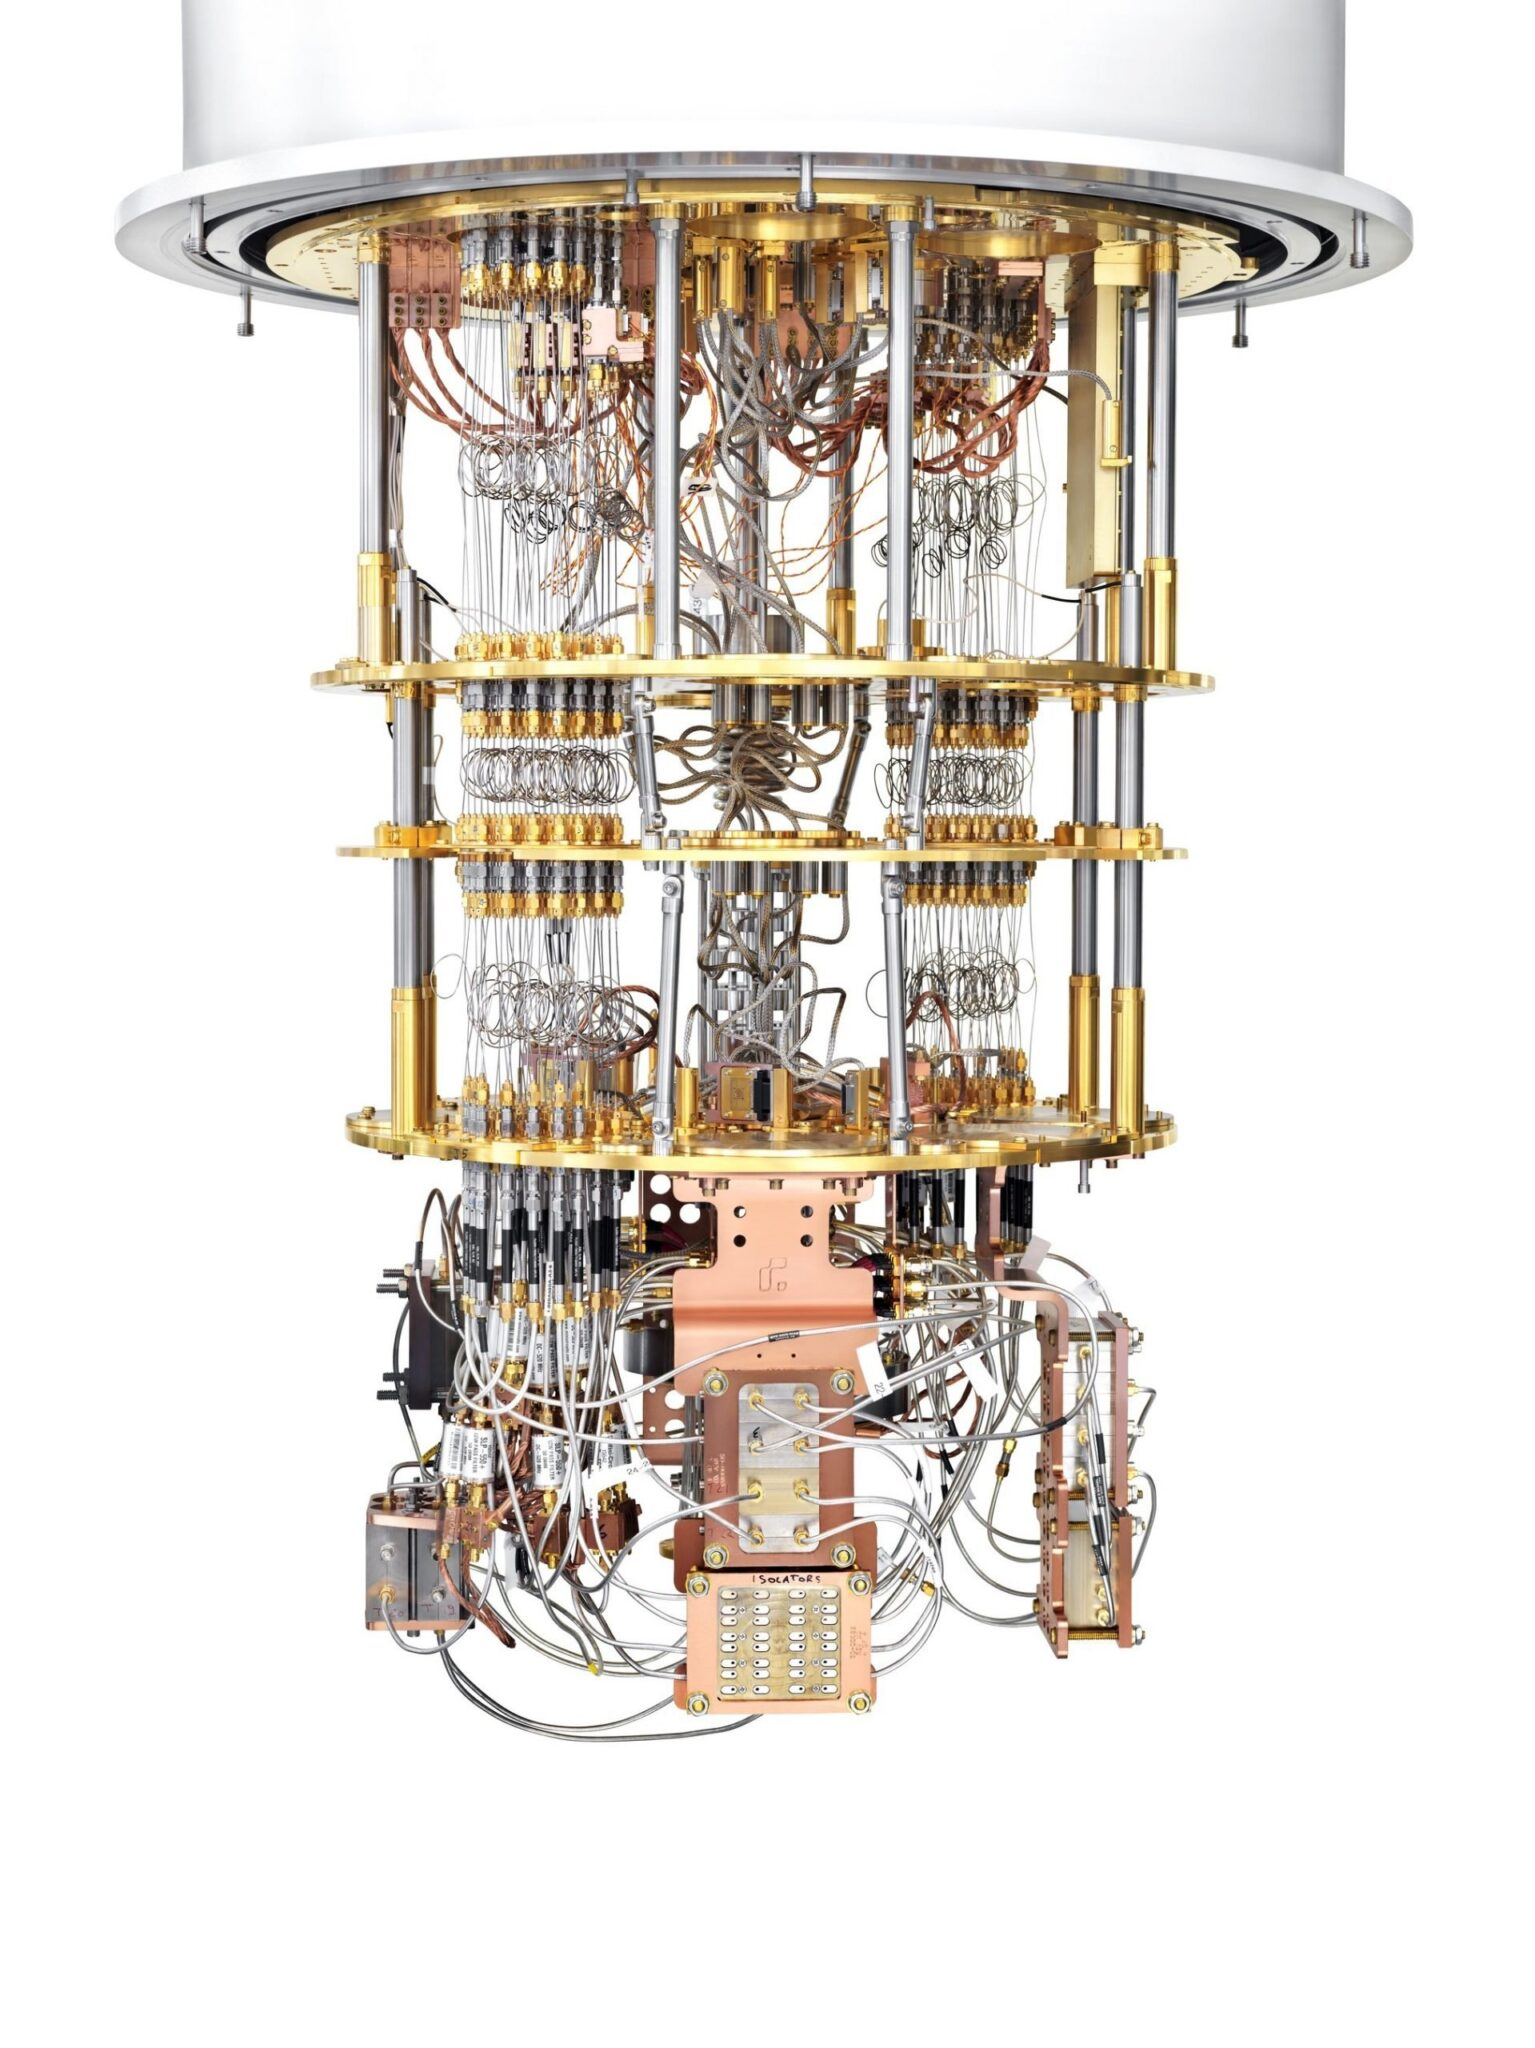
\includegraphics[height=0.85\textheight, width=\textwidth, keepaspectratio]{Rigetti-scaled-1535x2048.jpeg}
        \vfill
      \end{column}

    \begin{column}{0.35\textwidth}
        \small % Slightly smaller text often looks better in narrow columns
        \centering
        Quantum Computers leverage principles of quantum mechanics to perform some computational tasks much more efficiently.
        \newline
        \begin{itemize}
            \item Superposition
            \item Entanglement
            \item Interference
            \item Reversibility
        \end{itemize}
    \end{column}
    \hfill

\end{columns}
\end{frame}

%%%% Page 3 -- Why Quantum Computing?
\begin{frame}
\frametitle{Why Quantum Computing?}
\centering
\vfill

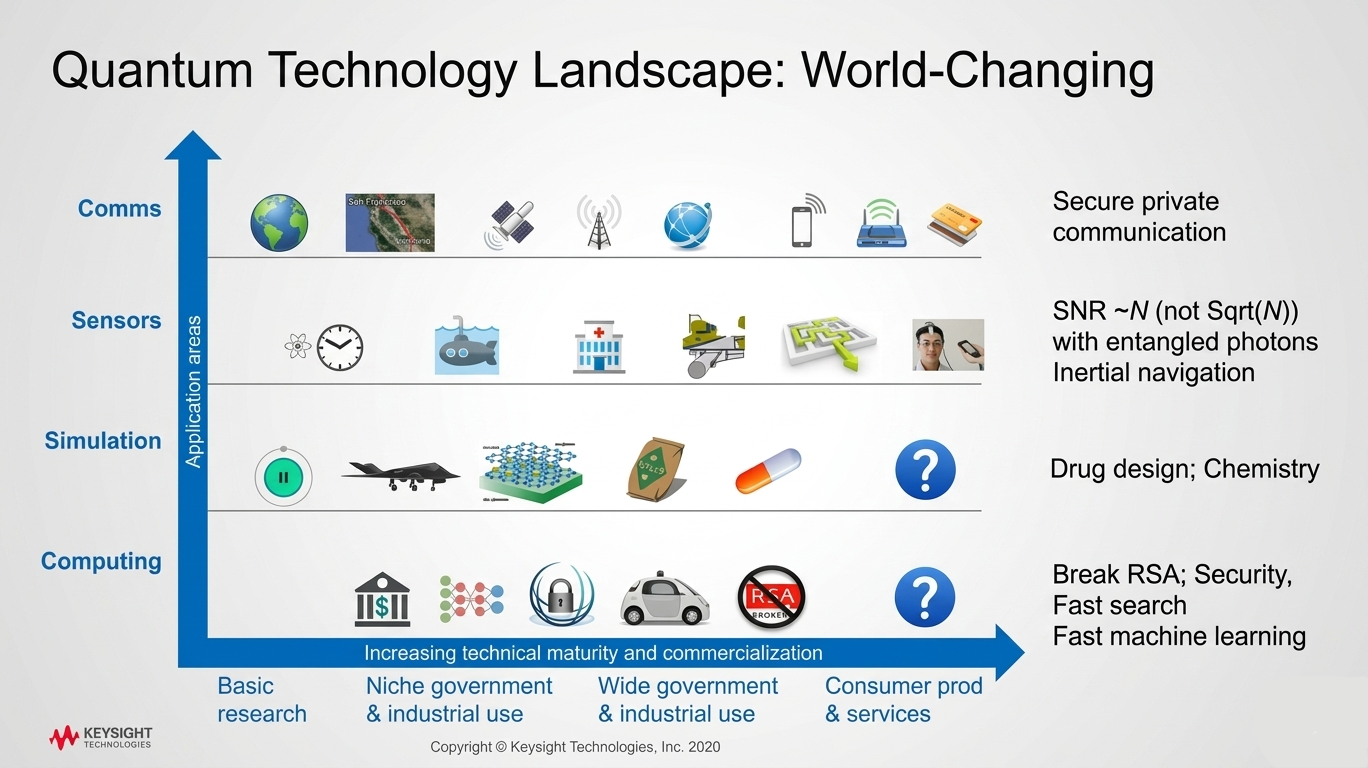
\includegraphics[height=0.75\textheight, width=\textwidth, keepaspectratio]{quantumSolutions.png}

\vfill 

\raggedleft
{\tiny Source: Dr. David Root, \textit{IEEE Microwave Theory and Technology Society}}

\end{frame}

%% Extra page to help development at so i can scroll and there is enough room for me to breath
\begin{frame}

\end{frame}


\end{document}
